Across the 10 confusable-class groups (22 images), the model misclassified
5 images (23\%). Table~\ref{tab:predictions} lists every prediction; errors
are bolded.

\begin{table}[h]
\centering
\small
\begin{tabular}{lllr}
\toprule
Group & Image & Predicted label & Conf. \\
\midrule
dogs\_husky\_malamute & malamute & malamute & 0.89 \\
dogs\_husky\_malamute & husky & \textbf{Tibetan mastiff} & 0.53 \\
cats\_tabby\_egyptian & egyptian\_cat & Egyptian cat & 0.87 \\
cats\_tabby\_egyptian & tabby\_cat & \textbf{Egyptian cat} & 0.46 \\
cats\_tabby\_egyptian & tiger\_cat & \textbf{tabby cat} & 0.33 \\
birds\_jay\_magpie & jay & jay & 0.92 \\
birds\_jay\_magpie & magpie & magpie & 0.87 \\
sharks & great\_white\_shark & great white shark & 0.92 \\
sharks & tiger\_shark & tiger shark & 0.88 \\
big\_cats & leopard & leopard & 0.84 \\
big\_cats & jaguar & \textbf{cougar} & 0.83 \\
foxes & red\_fox & red fox & 0.77 \\
foxes & kit\_fox & \textbf{grey fox} & 0.73 \\
foxes & grey\_fox & grey fox & 0.83 \\
elephants & indian\_elephant & Indian elephant & 0.81 \\
elephants & african\_elephant & African elephant & 0.92 \\
bears & american\_black\_bear & American black bear & 0.88 \\
bears & brown\_bear & brown bear & 0.92 \\
terriers & yorkshire\_terrier & Yorkshire terrier & 0.77 \\
terriers & silky\_terrier & silky terrier & 0.90 \\
retrievers & golden\_retriever & golden retriever & 0.92 \\
retrievers & labrador\_retriever & Labrador retriever & 0.93 \\
\bottomrule
\end{tabular}
\caption{Predicted label and confidence for all 22 test images, grouped by
confusable-class set. Bold rows are misclassifications.}
\label{tab:predictions}
\end{table}

Four of the five errors fall directly within the target confusable pair
(husky $\to$ Tibetan mastiff, tabby cat $\to$ Egyptian cat, tiger cat $\to$
tabby cat, kit fox $\to$ grey fox), and the fifth (jaguar $\to$ cougar) is a
visually similar spotted/tan big cat outside the intended pair -- consistent
with our hypothesis that errors cluster among classes sharing fur pattern
and body shape rather than occurring at random.

\subsection{Misclassified examples}

\begin{figure}[h]
\centering
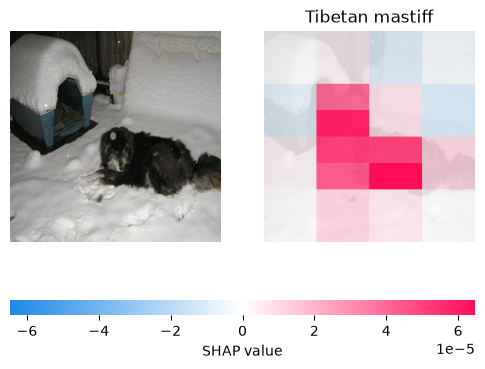
\includegraphics[width=0.7\textwidth]{figures/shap_husky.png}
\caption{Husky misclassified as Tibetan mastiff (conf.\ 0.53).}
\label{fig:husky}
\end{figure}

For the husky image (Figure~\ref{fig:husky}), SHAP attribution concentrates
on the dog's body and head rather than the snowy background, yet the model
still predicts Tibetan mastiff. The image is dark and the dog's fur is
mostly in shadow, so the region SHAP identifies as important is correct
(the dog, not the background) but the fine-grained texture cues that would
separate a husky from a mastiff -- pointed ears, mask-like facial
markings -- are not resolvable in this lighting.

\begin{figure}[h]
\centering
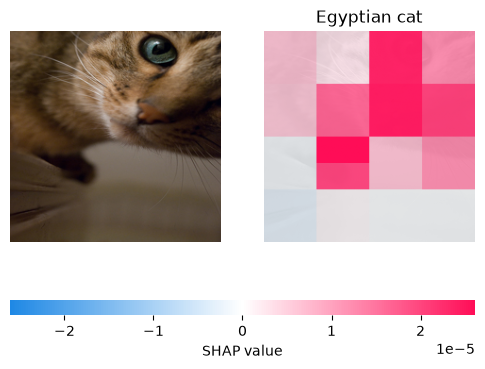
\includegraphics[width=0.7\textwidth]{figures/shap_tabby_cat.png}
\caption{Tabby cat misclassified as Egyptian cat (conf.\ 0.46).}
\label{fig:tabby}
\end{figure}

For the tabby cat image (Figure~\ref{fig:tabby}), attribution concentrates
tightly on the face and muzzle, and the model predicts Egyptian cat -- the
sibling class that shares the same facial spotting pattern. Here the model
is attending to exactly the right region (the face), but the tabby's facial
striping and the Egyptian cat's facial spotting are similar enough at this
crop that the region alone does not disambiguate the two classes.

\begin{figure}[h]
\centering
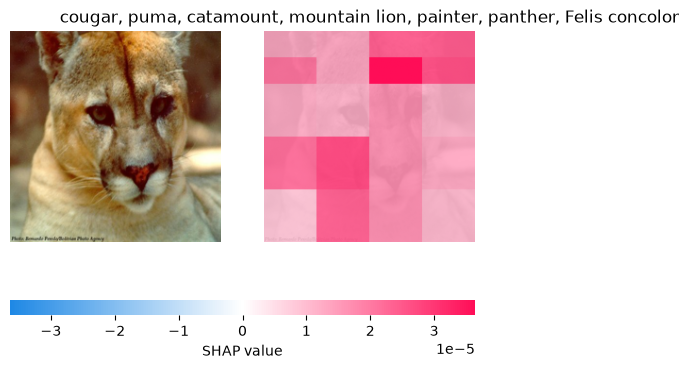
\includegraphics[width=0.7\textwidth]{figures/shap_jaguar.png}
\caption{Jaguar misclassified as cougar (conf.\ 0.83).}
\label{fig:jaguar}
\end{figure}

The jaguar image (Figure~\ref{fig:jaguar}) is the clearest case of a missing
cue. Attribution again falls on the animal's face, correctly ignoring the
background, but the jaguar's rosette pattern is barely visible in this
close, evenly lit headshot. With the coat pattern effectively absent from
the model's evidence, it falls back on face shape and coloring, which is
shared with the plain-coated cougar. This mirrors a correctly classified
leopard image (Figure~\ref{fig:leopard}, Section~\ref{sec:correct}), where
the same face-centered attribution pattern appears but the rosettes are
clearly visible, and the model gets the label right.

\begin{figure}[h]
\centering
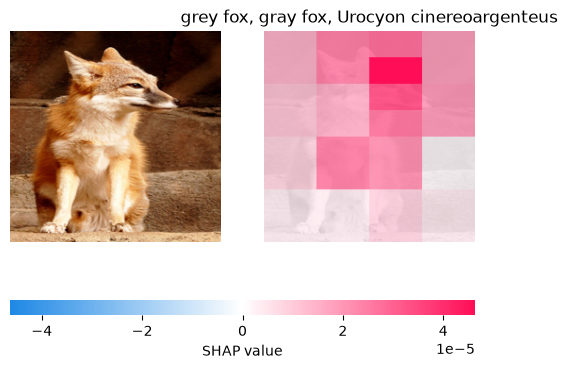
\includegraphics[width=0.7\textwidth]{figures/shap_kit_fox.png}
\caption{Kit fox misclassified as grey fox (conf.\ 0.73).}
\label{fig:kitfox}
\end{figure}

For the kit fox image (Figure~\ref{fig:kitfox}), attribution spreads across
the head and body rather than isolating the ears -- the feature most
diagnostic of kit fox (unusually large ears relative to head size). Because
the explainer's blur-based superpixels are coarse (roughly $4\times4$
regions per image at \texttt{max\_evals=100}), the ears are not resolved
as a separate region from the rest of the head, so at this resolution alone
we could not tell whether the model ignores ear size or simply cannot have
that cue isolated for it. Section~\ref{sec:highres} re-runs SHAP on this
image (and the other four errors) at \texttt{max\_evals=400} specifically
to resolve this question.

\begin{figure}[h]
\centering
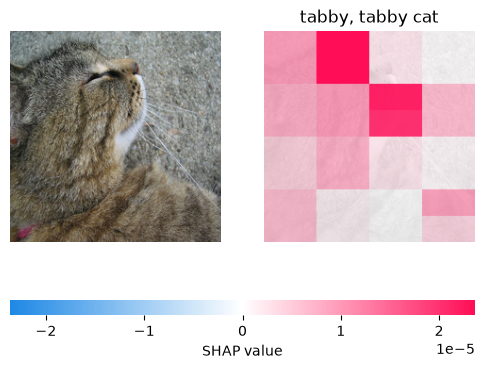
\includegraphics[width=0.7\textwidth]{figures/shap_tiger_cat.png}
\caption{Tiger cat misclassified as tabby cat (conf.\ 0.33, the lowest
confidence of any prediction in our set).}
\label{fig:tigercat}
\end{figure}

The tiger cat image (Figure~\ref{fig:tigercat}) is the model's least
confident prediction overall. Attribution again lands on the cat's face and
ear, correctly avoiding the background, but the crop shows only striped fur
without the cat's full body pattern -- tiger cat and tabby cat are two
ImageNet labels for closely related striped coat patterns, and at this crop
angle there is little in the visible texture to separate them. The low
confidence (0.33, versus 0.7-0.9 for most other predictions in our set)
suggests the model itself is registering this ambiguity rather than
confidently picking the wrong class.

\subsection{Correctly classified examples for contrast}
\label{sec:correct}

\begin{figure}[h]
\centering
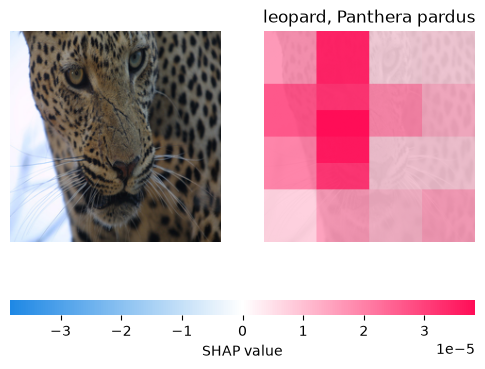
\includegraphics[width=0.7\textwidth]{figures/shap_leopard.png}
\caption{Leopard correctly classified (conf.\ 0.84).}
\label{fig:leopard}
\end{figure}

\begin{figure}[h]
\centering
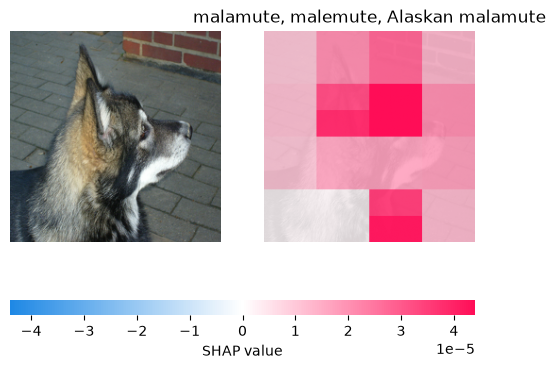
\includegraphics[width=0.7\textwidth]{figures/shap_malamute.png}
\caption{Malamute correctly classified (conf.\ 0.89).}
\label{fig:malamute}
\end{figure}

In the leopard image (Figure~\ref{fig:leopard}), SHAP attribution is
concentrated on the face, where the rosette pattern is clearly visible and
well lit -- the same region attended to in the misclassified jaguar image,
but here the discriminating texture is actually present in the crop, and
the model gets the label right. In the malamute image
(Figure~\ref{fig:malamute}), attribution concentrates on the head and ear
region, where breed-distinguishing features (ear shape, facial mask) are
visible in good lighting.

Taken together, these examples support a consistent pattern: in both
correct and incorrect predictions, SHAP attribution falls on the animal's
head or body rather than the background. The difference between correct
and incorrect predictions in our error cases is less about \emph{where} the
model looked and more about whether the distinguishing texture cue was
actually visible and salient within that region.

\subsection{High-resolution refinement of the 5 misclassified cases}
\label{sec:highres}

The baseline pass above uses \texttt{max\_evals=100}, which yields a coarse
$\sim4\times4$ superpixel grid per image (Section~\ref{sec:limitations}).
This leaves open the question raised for the kit fox and cat cases above:
is attribution spread across the head because the model genuinely does not
privilege the fine-grained discriminative feature (ears, facial pattern),
or because SHAP's grid is too coarse to isolate that feature as its own
region? To answer this directly, we re-ran \texttt{code/run\_shap.py} in
\texttt{highres-errors} mode, which reads \texttt{logs/shap\_results.json},
isolates exactly the 5 misclassified images (husky, tabby\_cat, tiger\_cat,
jaguar, kit\_fox), and recomputes SHAP attribution for each at
\texttt{max\_evals=400} -- a $\sim4\times$ finer superpixel grid -- leaving
the other 17 images and the baseline figures untouched. The refined
predictions and confidences are unchanged from the baseline pass (as
expected, since \texttt{max\_evals} affects only the SHAP approximation,
not the underlying classifier), which lets us compare the two attribution
maps for the same prediction directly.

\begin{figure}[h]
\centering
\begin{minipage}{0.48\textwidth}
\centering
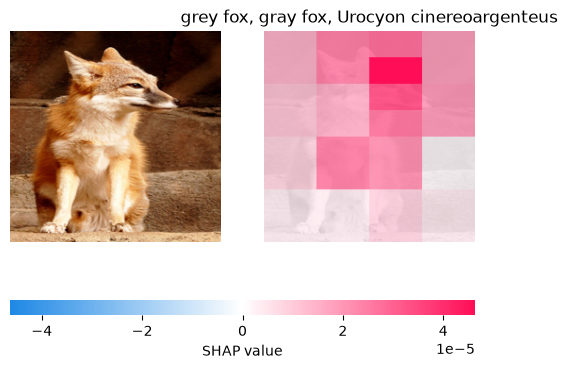
\includegraphics[width=\textwidth]{figures/shap_kit_fox.png}
\caption*{\texttt{max\_evals=100} (baseline)}
\end{minipage}
\hfill
\begin{minipage}{0.48\textwidth}
\centering
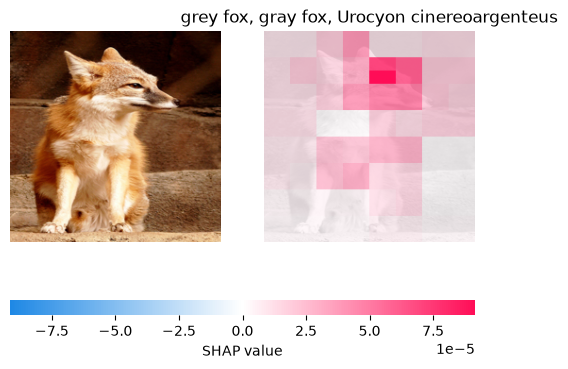
\includegraphics[width=\textwidth]{figures/shap_highres_kit_fox.png}
\caption*{\texttt{max\_evals=400} (refined)}
\end{minipage}
\caption{Kit fox misclassified as grey fox: baseline vs.\ refined SHAP
resolution.}
\label{fig:kitfox-highres}
\end{figure}

\textbf{Kit fox (Figure~\ref{fig:kitfox-highres}).} At \texttt{max\_evals=400}
the finer grid pulls attribution weight noticeably away from the lower body
and concentrates it into a tight, high-intensity cluster over the head and
ear region -- the single most saturated cell in the refined map sits
directly on the ear/head area, versus a more diffuse head-and-shoulder
patch in the baseline. This is a resolution artifact of exactly the kind
the limitations section flagged: at \texttt{max\_evals=100} the model's
actual attention to the ear region was present but blended into a larger
superpixel, and the coarse grid made it look like the model was not
privileging that feature at all. At \texttt{max\_evals=400}, the ear region
is attended to more strongly than the rest of the head, which does support
the model registering the ear as informative -- so the error is better
explained by an under-confident or noisy signal (0.73 for grey fox instead
of kit fox) than by the model ignoring the feature outright.

\begin{figure}[h]
\centering
\begin{minipage}{0.48\textwidth}
\centering
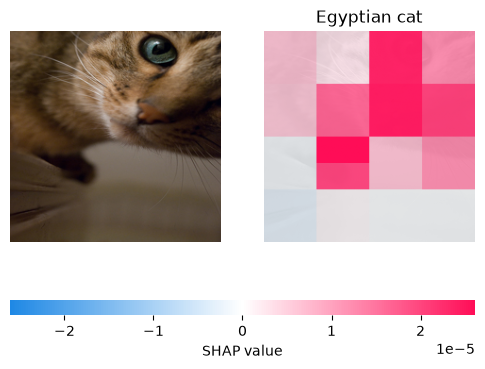
\includegraphics[width=\textwidth]{figures/shap_tabby_cat.png}
\caption*{\texttt{max\_evals=100} (baseline)}
\end{minipage}
\hfill
\begin{minipage}{0.48\textwidth}
\centering
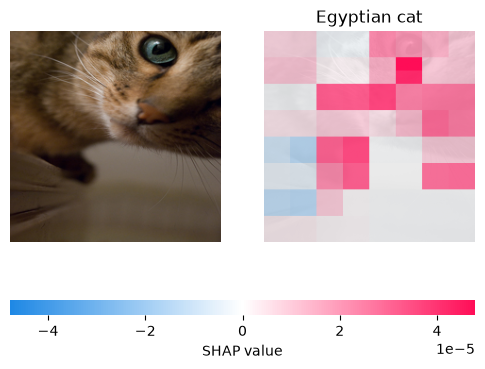
\includegraphics[width=\textwidth]{figures/shap_highres_tabby_cat.png}
\caption*{\texttt{max\_evals=400} (refined)}
\end{minipage}
\caption{Tabby cat misclassified as Egyptian cat: baseline vs.\ refined SHAP
resolution.}
\label{fig:tabby-highres}
\end{figure}

\begin{figure}[h]
\centering
\begin{minipage}{0.48\textwidth}
\centering
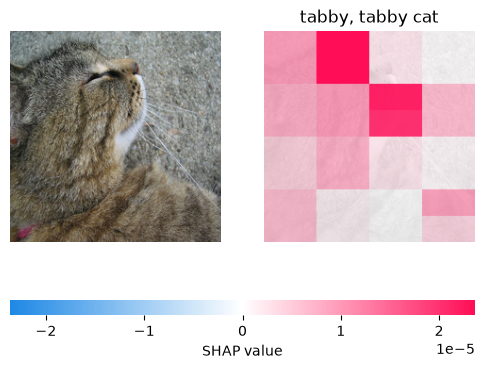
\includegraphics[width=\textwidth]{figures/shap_tiger_cat.png}
\caption*{\texttt{max\_evals=100} (baseline)}
\end{minipage}
\hfill
\begin{minipage}{0.48\textwidth}
\centering
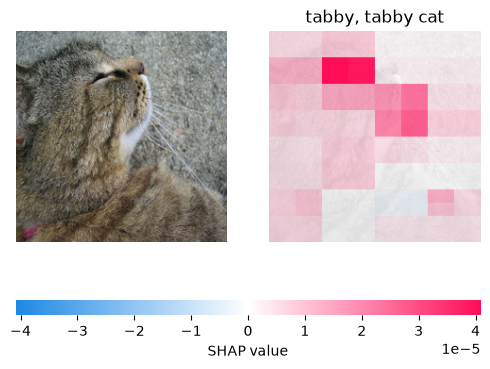
\includegraphics[width=\textwidth]{figures/shap_highres_tiger_cat.png}
\caption*{\texttt{max\_evals=400} (refined)}
\end{minipage}
\caption{Tiger cat misclassified as tabby cat: baseline vs.\ refined SHAP
resolution.}
\label{fig:tigercat-highres}
\end{figure}

\textbf{Tabby cat and tiger cat (Figure~\ref{fig:tabby-highres} and
Figure~\ref{fig:tigercat-highres}).} For both cat images, the refined map
reproduces the same face-and-muzzle attribution pattern as the baseline,
at finer spatial detail -- no new region (e.g.\ ear shape, body coat) is
revealed as important once resolved. This is the opposite outcome from the
kit fox case: here, more resolution does not surface a previously-hidden
feature, which is evidence that the baseline result was already an
accurate summary of what the model was using, not an artifact of an
under-resolved grid. The remaining ambiguity is therefore attributable to
the model's failure to disambiguate two closely related facial patterns
within the region it correctly attends to, not to SHAP failing to isolate
that region.

\begin{figure}[h]
\centering
\begin{minipage}{0.48\textwidth}
\centering
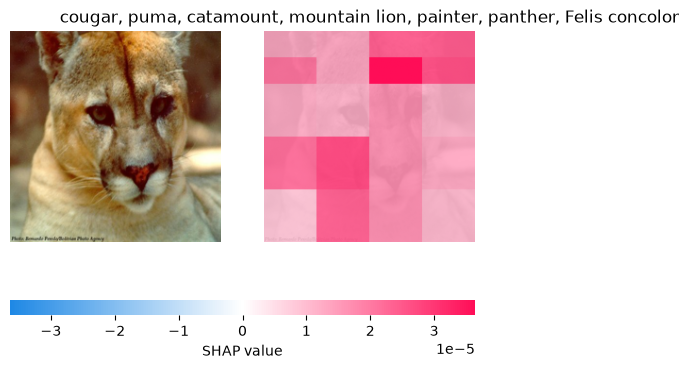
\includegraphics[width=\textwidth]{figures/shap_jaguar.png}
\caption*{\texttt{max\_evals=100} (baseline)}
\end{minipage}
\hfill
\begin{minipage}{0.48\textwidth}
\centering
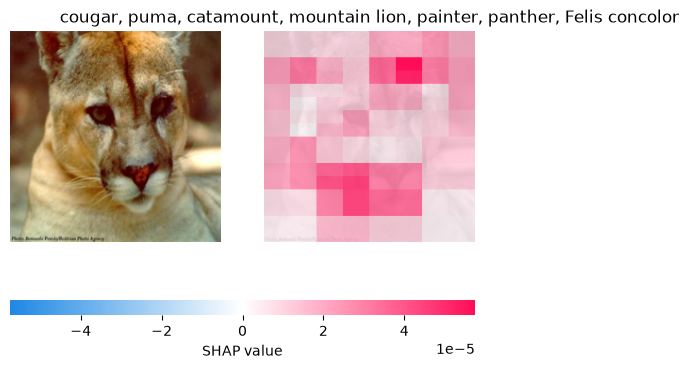
\includegraphics[width=\textwidth]{figures/shap_highres_jaguar.png}
\caption*{\texttt{max\_evals=400} (refined)}
\end{minipage}
\caption{Jaguar misclassified as cougar: baseline vs.\ refined SHAP
resolution.}
\label{fig:jaguar-highres}
\end{figure}

\textbf{Jaguar (Figure~\ref{fig:jaguar-highres}).} The refined map again
reproduces the baseline's face-centered attribution at finer granularity,
with no new attention to a region where a rosette pattern might be hiding.
This corroborates the baseline reading: the coat pattern is not merely
under-resolved by SHAP, it is genuinely close to absent from this crop, and
higher resolution does not manufacture attribution to it.

\begin{figure}[h]
\centering
\begin{minipage}{0.48\textwidth}
\centering
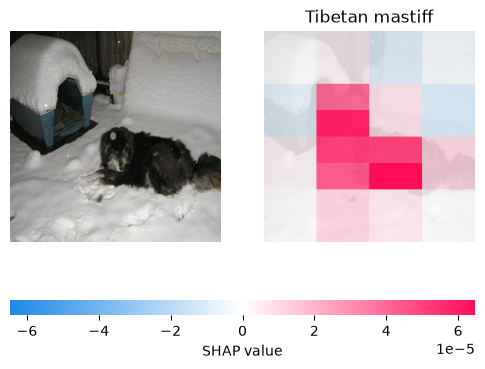
\includegraphics[width=\textwidth]{figures/shap_husky.png}
\caption*{\texttt{max\_evals=100} (baseline)}
\end{minipage}
\hfill
\begin{minipage}{0.48\textwidth}
\centering
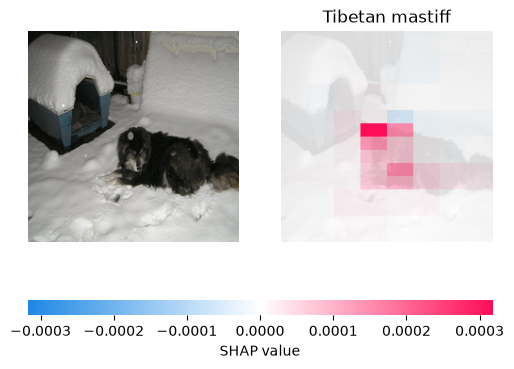
\includegraphics[width=\textwidth]{figures/shap_highres_husky.png}
\caption*{\texttt{max\_evals=400} (refined)}
\end{minipage}
\caption{Husky misclassified as Tibetan mastiff: baseline vs.\ refined SHAP
resolution.}
\label{fig:husky-highres}
\end{figure}

\textbf{Husky (Figure~\ref{fig:husky-highres}).} The refined map keeps
attribution on the dog's torso and does not shift weight toward the head or
ears even at $4\times$ the resolution. Given that the husky's head is
visible but heavily backlit and in shadow in this photo, this is consistent
with our reading in Section~\ref{sec:limitations}: the limiting factor here
is that the discriminating texture (pointed ears, facial mask) is not
well-lit in the source photo, not that SHAP's grid was too coarse to find
it.

\textbf{Summary.} Higher resolution changes the picture for one of the five
error cases (kit fox) and confirms the baseline reading for the other four
(tabby cat, tiger cat, jaguar, husky). This closes the open question from
the baseline results: the flat or diffuse attribution we saw at
\texttt{max\_evals=100} was, in the kit fox case, a genuine artifact of an
under-resolved superpixel grid masking attention that the model did in fact
place on the ears; in the other four cases it was not an artifact, and the
model's failure to use the discriminating cue is a property of the
model/image pair rather than of our explainer's resolution. We revisit the
implications of this for the paper's open question in
Section~\ref{sec:discussion-highres}.
